\chapter{Analisis}
\label{chap:analisis}

\section{Analisis Sistem Masa Kini}
    Analisis sistem yang digunakan pada saat ini di lab komputasi akan dimulai
    dengan menganalisis alur pelaksanaan ujian terlebih dahulu. Kemudian
    dilanjutkan dengan melakukan penyebaran kuisioner untuk mendapatkan
    informasi lebih lanjut tentang masalah yang tidak teridentifikasi pada saat
    survei pelaksanaan ujian.
    
    Kedua sumber informasi tersebut kemudian akan dianalisis untuk membuat
    usulan fitur baru yang akan diimplementasi pada sistem yang baru.

\subsection{Pelaksanaan Ujian}

    \begin{figure}[H]
        \centering
        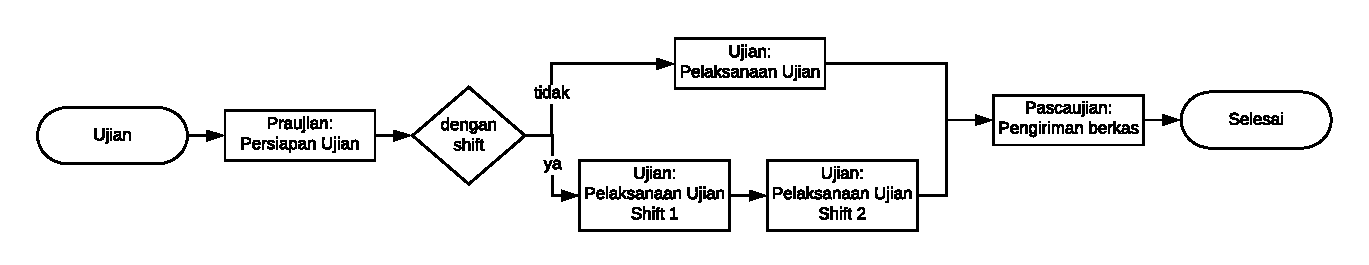
\includegraphics[width=0.75\paperwidth]{Gambar/flowchart/exam-flow-ujian.pdf}
        \caption{Diagram alur pelaksanaan ujian secara garis besar}
        \label{fig:flowchart-exam-outline}
    \end{figure}
    
    Analisis domain masalah dimulai dengan melakukan survei lapangan pada
    pelaksanaan ujian. Pada pelaksanaan ujian, terdapat tiga tahap penting yang
    akan dilalui oleh tiap peran. Pada Gambar \ref{fig:flowchart-exam-outline},
    proses ujian dimulai dengan tahap persiapan ujian. Kemudian pada tahap
    berikutnya terdapat pelaksanaan ujian bergantung pada ada atau tidaknya
    \textit{shift} pada ujian tersebut. Kemudian ditutup dengan pengiriman
    berkas ujian pada tahap pascaujian.
    
    \subsubsection{Praujian}
    
        \begin{figure}
            \centering
            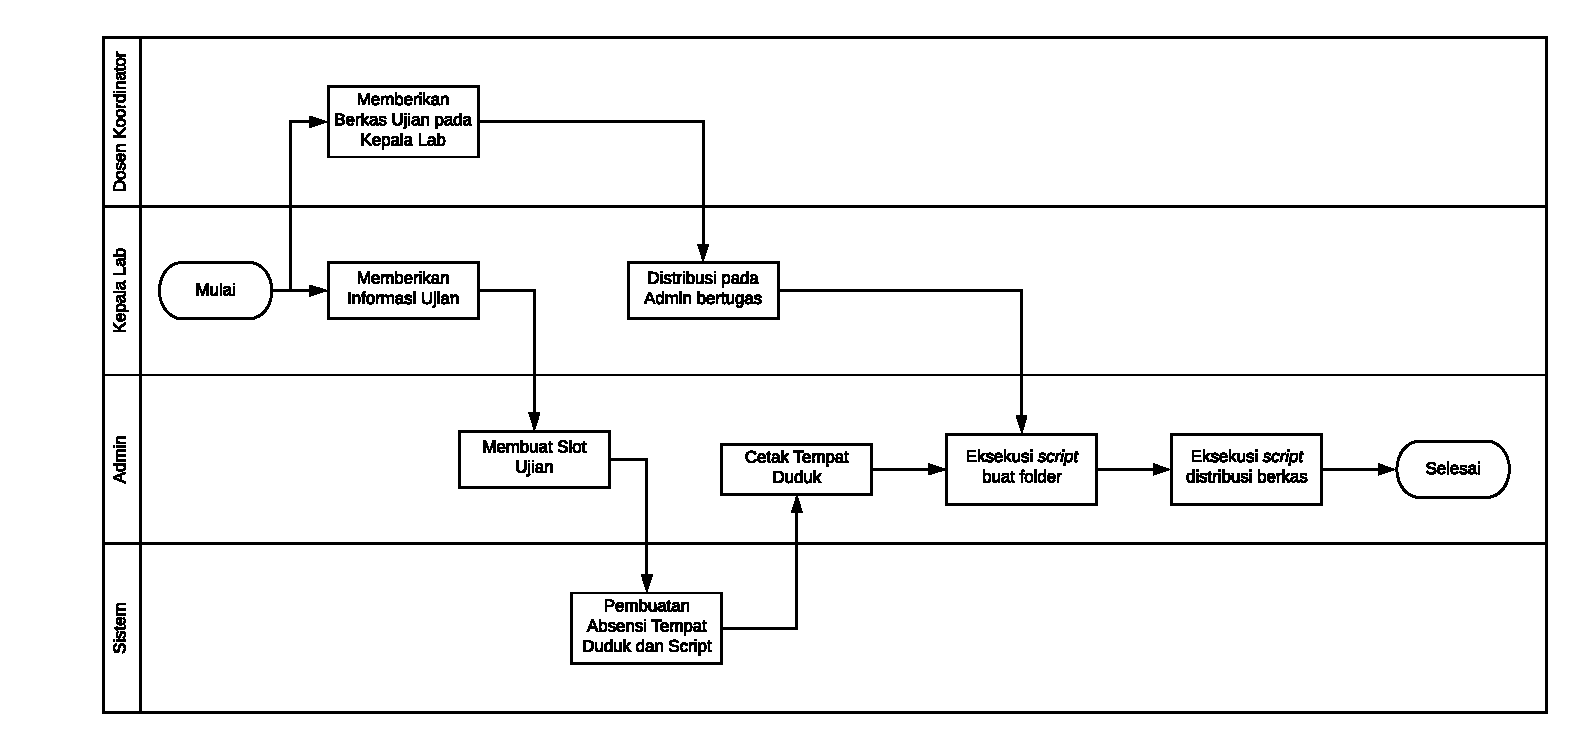
\includegraphics[width=0.75\paperwidth]{Gambar/flowchart/exam-flow-ujian-pra.pdf}
            \caption{Diagram alur detil persiapan ujian}
            \label{fig:flowchart-exam-preexam}
        \end{figure}
        
        Berdasarkan survei lapangan yang dilakukan, persiapan yang dilakukan
        untuk ujian dilakukan beberapa hari sebelum ujian dilaksanakan. Pada
        tahap ini pihak yang terlibat dalam pembuatan slot ujian adalah Admin
        dan Dosen. Alur praujian pada Gambar \ref{fig:flowchart-exam-outline}
        diperjelas pada Gambar \ref{fig:flowchart-exam-preexam} dengan
        mendetilkan masing-masing peran yang terlibat.
        
        
        Admin akan membuatkan slot ujian pada sistem Oxam, dan mengatur posisi
        tempat duduk sesuai dengan jumlah dan informasi ujian yang diberikan
        dari kepala lab. Sistem kemudian akan menghasilkan daftar tempat duduk
        yang telah diacak oleh sistem. Admin kemudian mencetak daftar tempat
        duduk tersebut untuk nantinya didistribusikan sesuai ruangannya. Dosen
        koordinator yang bertugas untuk membuat soal ujian akan memberikan
        berkas tersebut ke kepala lab. Berkas tersebut kemudian didistribusikan
        pada Admin yang bertugas untuk menjaga ujian.
        
        Sistem juga menghasilkan beberapa \textit{script} dengan fungsi sebagai
        berikut:
        \begin{itemize}
            \item Membuat folder lembar kerja untuk peserta pada masing-masing
            komputer yang telah dimasukkan pada sistem.
            \item Mendistribusikan berkas soal ujian dan berkas bantuan pada
            masing-masing komputer peserta.
            \item Mengambil alih pemilik berkas pada folder lembar kerja peserta
            pada masing-masing komputer.
        \end{itemize}
        
        Persiapan ujian lalu berlanjut pada eksekusi \textit{script} yang
        diberikan oleh aplikasi Oxam. Admin yang bertugas kemudian memasukan
        berkas-berkas ujian pada lokasi khusus di server \textit{deployment}.
        Kemudian script pembuatan folder dan distribusi berkas dieksekusi.
        \textit{Script} yang dieksekusi akan menghasilkan log yang
        menginformasikan keberhasilan pendistribusian berkas tersebut. Admin
        yang bertugas akan memperhatikan log tersebut dan melakukan hal-hal yang
        perlu dilakukan jika terdapat masalah pada log tersebut.
        
        Daftar tempat duduk akan didistribusikan pada pintu lobi dan pintu ruang
        ujian sesaat sebelum ujian dimulai.
    
    \subsubsection{Ujian}
        \begin{figure}
            \centering
            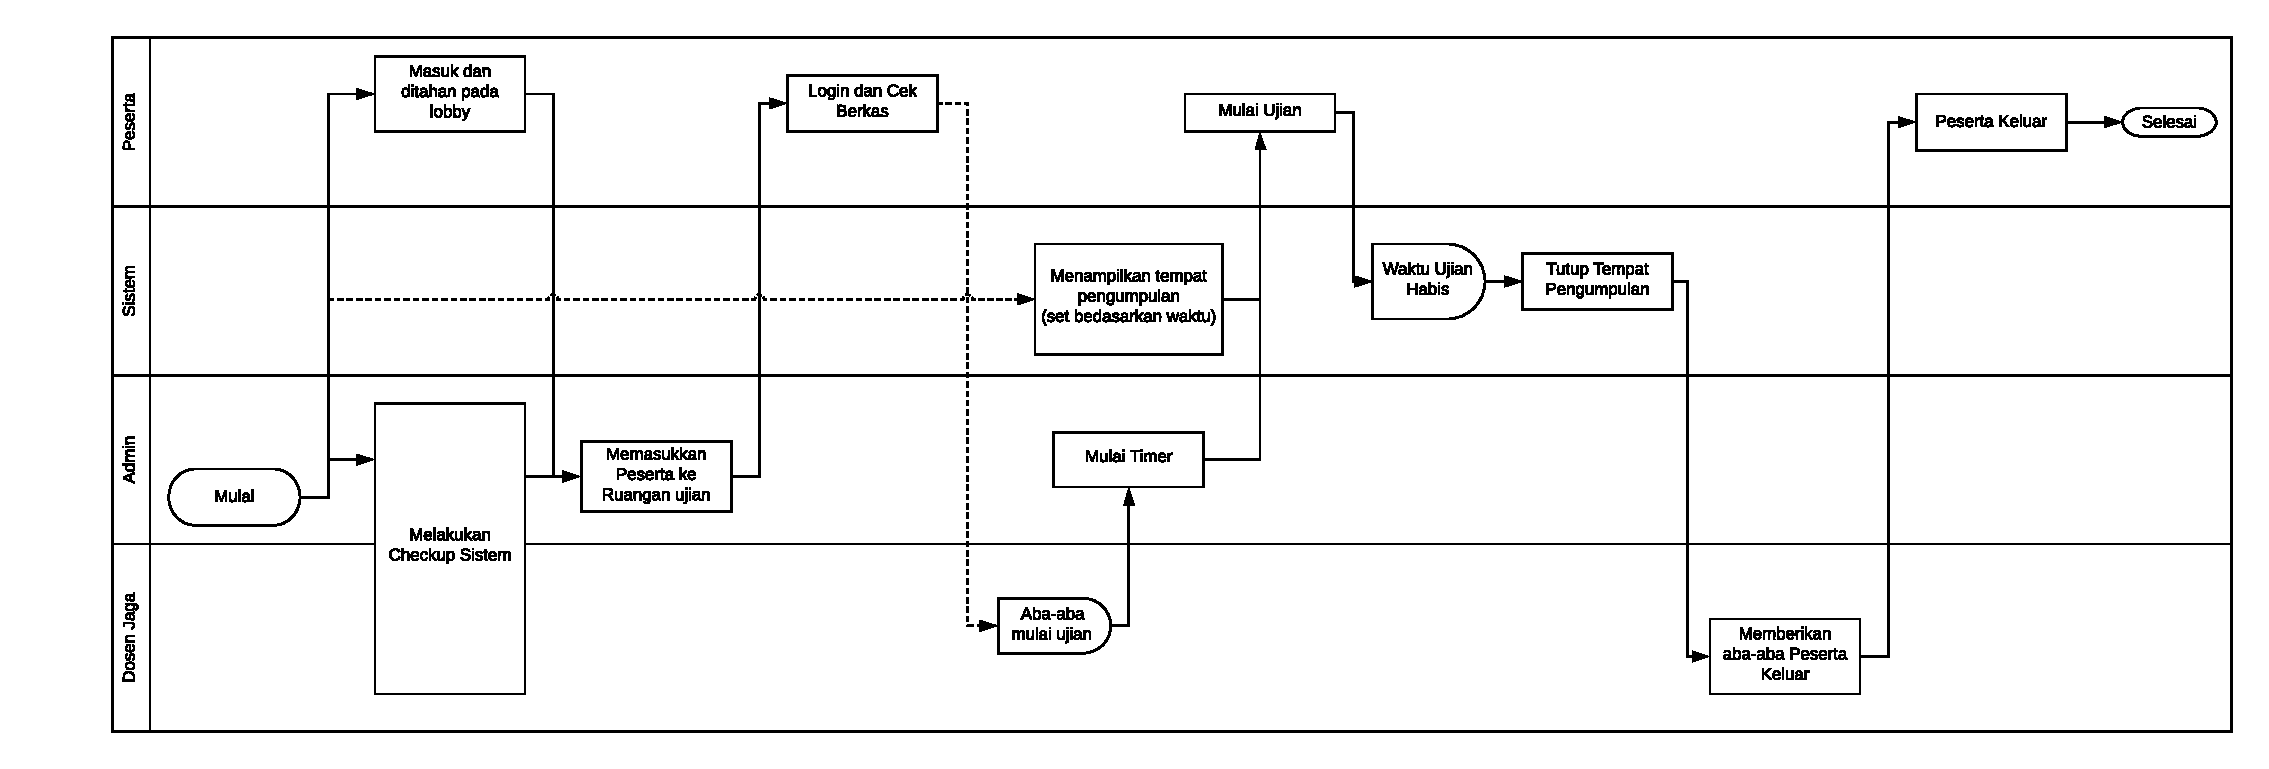
\includegraphics[width=0.75\paperwidth]{Gambar/flowchart/exam-flow-ujian-no-shift.pdf}
            \caption{Diagram alur ujian dengan tanpa shift}
            \label{fig:flowchart-exam-exam-noshift}
        \end{figure}
        % Admin menahan mahasiswa pada lobby
        Proses Ujian kemudian berlanjut pada hari pelaksanaan ujian tersebut
        diadakan. Alur pelaksanaan ujian pada diagram
        \ref{fig:flowchart-exam-outline}, dijelaskan dengan lebih mendetil pada
        diagram \ref{fig:flowchart-exam-exam-noshift}. Peserta yang telah
        diminta hadir 30 menit sebelumnya akan diarahkan untuk masuk dan
        menunggu pada lobi lab. Admin yang bertugas akan memastikan setiap
        peserta yang akan memasuki ruangan ujian telah membawa kartu mahasiswa.
        Dosen ditugaskan untuk menjaga akan melakukan persiapan ujian seperti
        membagikan kertas buram dan sterilisasi ruangan.
        
        % Admin melakukan checkup sekali lagi 
        Sementara itu, Admin beserta dengan dosen yang bertugas untuk menjaga
        selama ujian akan melakukan \textit{check up} terakhir untuk memastikan
        bahwa distribusi soal tidak bermasalah. \textit{Check up} dilakukan
        dengan bantuan daftar check yang telah dibuat Kepala Lab. Pemasangan
        timer dilakukan pada tahap ini.
        
        % Admin memasukan mahasiswa pada ruang ujian
        Setelah \textit{check up} selesai dan tidak terdapat masalah, admin akan
        membuka sekat pemisah ruang lobi dan ruang ujian. Peserta kemudian masuk
        ke ruangan ujian, dan dipersilahkan duduk sesuai dengan daftar tempat
        duduk yang telah didistribusikan.
        
        % Mahasiswa dipersilahkan login dan melakukan cek berkas bantuan dan
        % ujian (cek ada atau tidak)
        Peserta yang sudah duduk kemudian dipersilahkan untuk segera login dan
        melakukan cek pada berkas ujian tersebut. Peserta yang sudah siap akan
        menunggu aba-aba dari dosen penjaga untuk memulai ujian. Admin yang
        bertugas akan bersiap pada komputer proyektor untuk memulai timer.
        
        % Dosen jaga memberikan aba-aba, Admin start timer & Standby, Mahasiswa
        % mulai ujian
        Pada saat dosen penjaga memberikan aba-aba untuk memulai ujian, admin
        yang bertugas akan memulai timer dan mahasiswa dapat memulai ujian. Slot
        untuk mengumpulkan tempat jawaban akan muncul pada waktu yang
        ditentukan. Peserta ujian dapat melakukan pengunggahan berkas jawaban ke
        portal web dari sistem yang telah dibuka.
        
        % Waktu habis, Dosen jaga beri aba-aba untuk keluar.
        Pada saat waktu ujian telah habis, dosen yang berjaga akan memberikan
        aba-aba untuk peserta menghentikan pengerjaan ujian. Lalu dilanjutkan
        dengan memberikan aba-aba untuk mengeluarkan peserta dari ruangan.
    
    \subsubsection{Ujian dengan shift}
        \begin{figure}
            \centering
            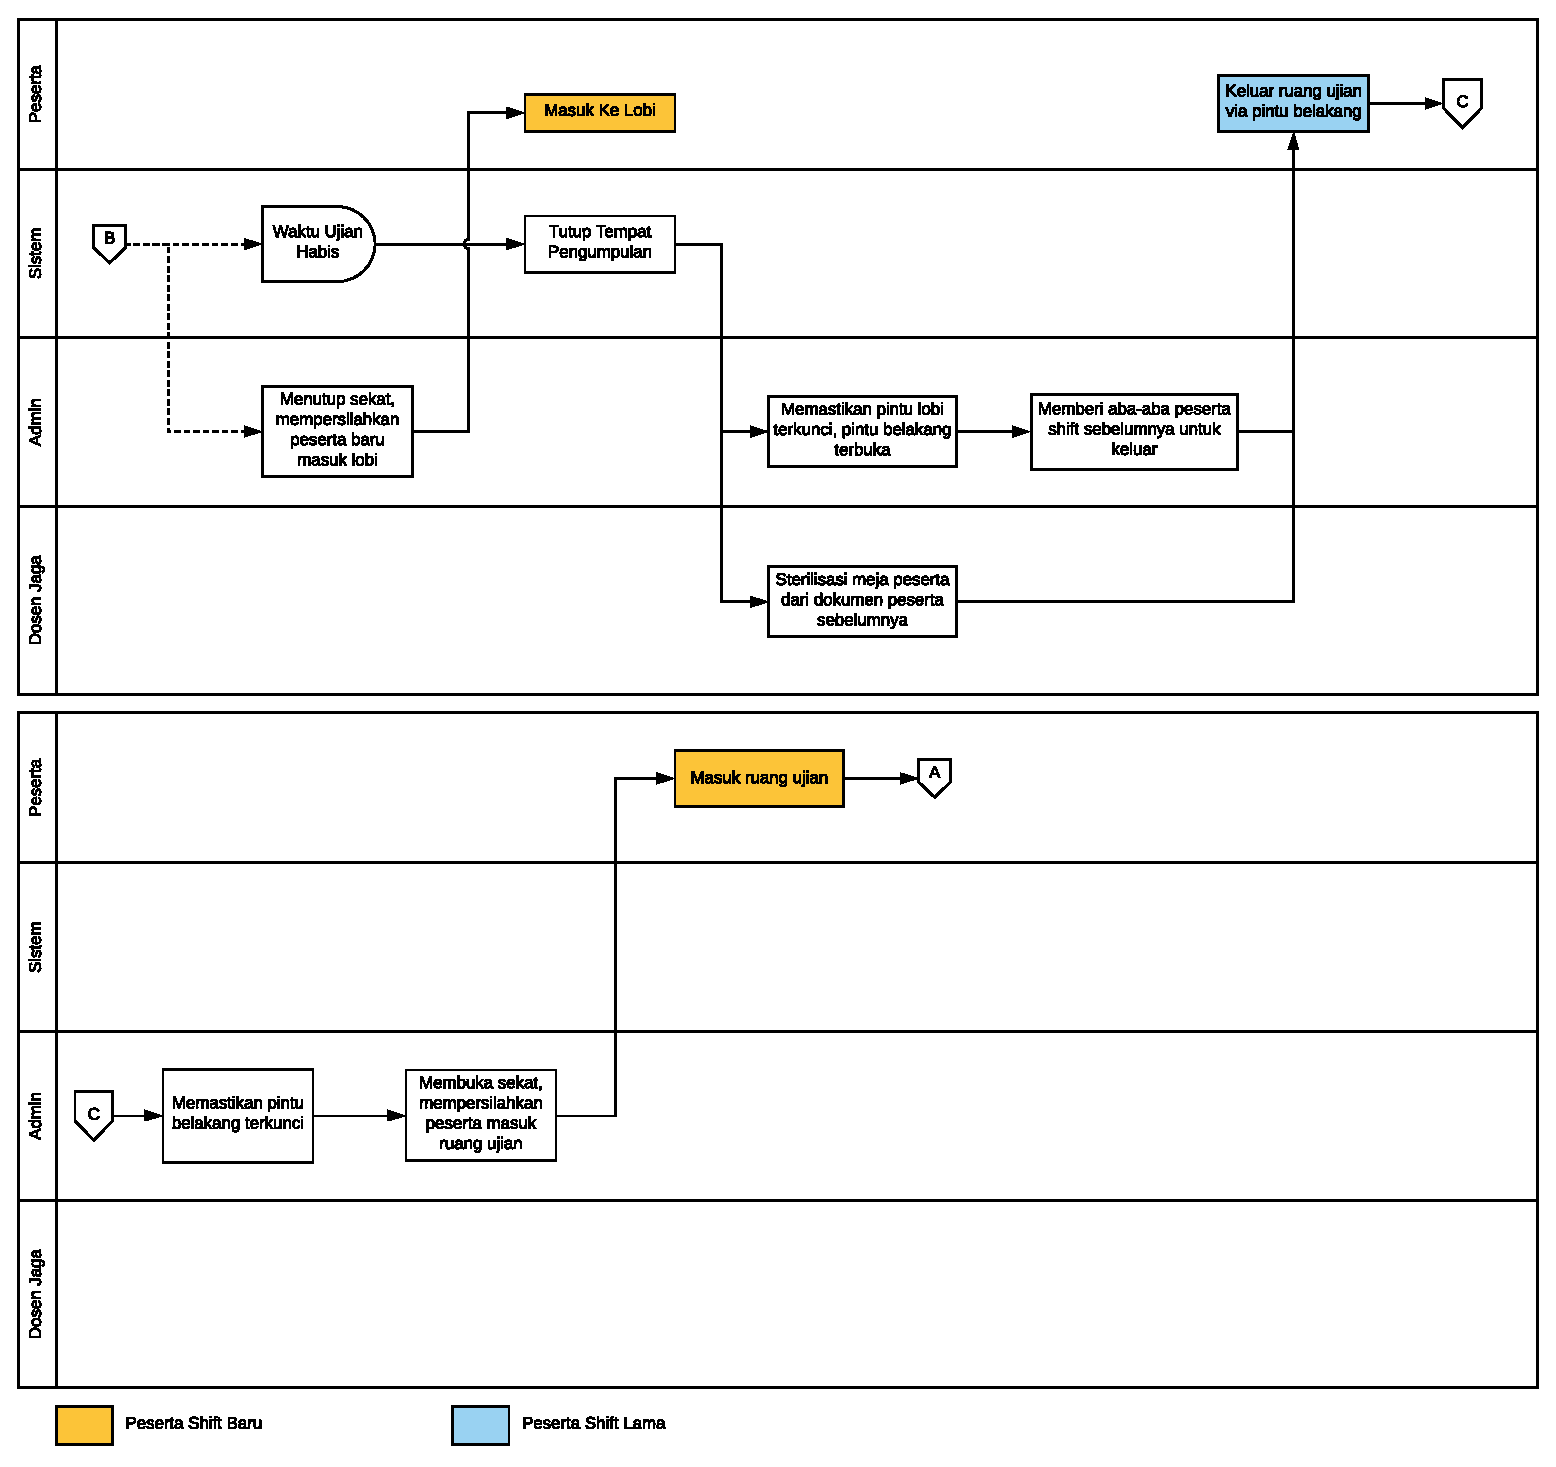
\includegraphics[width=0.75\paperwidth]{Gambar/flowchart/exam-flow-ujian-shift.pdf}
            \caption{Diagram alur ujian dengan shift}
            \label{fig:flowchart-exam-exam-with-shift}
        \end{figure}
        % Admin memastikan pintu lobby terkunci, sekat menuju ruangan tertutup
        Ujian dengan shift memiliki sedikit perbedaan dalam pelaksanaan ujian.
        Dapat dilihat pada diagram \ref{fig:flowchart-exam-exam-with-shift},
        pebedaan pelaksanaan ini terdapat pada proses memasukan dan mengeluarkan
        peserta antar shift). Pelaksanaan ujian dengan shift ini akan
        mengutamakan isolasi peserta dari peserta yang sudah mengerjakan soal
        ujian. Isolasi tersebut berguna untuk mencegah kecurangan dengan
        membagikan jawaban atau informasi tentang soal pada peserta yang akan
        ujian. Isolasi tersebut dimulai sesaat sebelum waktu ujian pada peserta
        shift sebelumnya telah habis. Admin akan datang pada ruangan untuk
        menahan peserta yang sedang ujian untuk tidak keluar terlebih dahulu.
        Admin lainnya akan memasukan peserta baru ke dalam lobi yang terisolasi.
        Sekat yang memisahkan ruangan lobi dan peserta akan dipasang kembali,
        menahan peserta shift baru tetap di lobi.
        
        % Admin memberikan aba-aba untuk peserta shift sebelumnya keluar lewat
        % pintu belakang
        Saat timer tanda waktu ujian telah habis berbunyi, Admin akan
        berkoordinasi memastikan bahwa pintu lobi telah dikunci dan pintu
        belakang telah dibuka. Admin kemudian akan memberikan aba-aba untuk
        mengeluarkan peserta shift sebelumnya melalui pintu belakang. Dosen yang
        berjaga kemudian melakukan persiapan ujian kembali dengan mensterilkan
        meja peserta dari berkas lama peserta sebelumnya, dan membagikan soal.
        
        % Admin mengunci pintu belakang, Admin membuka sekat menuju ruangan,
        % mempersilahkan peserta masuk
        Setelah peserta ujian pada shift sebelumnya telah keluar sepenuhnya dari
        ruang ujian, Admin akan mengunci pintu belakang, mengisolasi seluruh
        peserta shift baru. Sekat kemudian dibuka dan peserta ujian pada shift
        baru dipersilahkan masuk ke dalam ruangan ujian. Kemudian ujian
        dilakukan sesuai dengan prosedur pelaksanaan ujian seperti biasa.
    
    \subsubsection{Pascaujian}
        % take own
        Alur ujian berikutnya yang dilalui adalah proses manajemen berkas
        jawaban ujian. Lembar kerja peserta pada komputer yang digunakan
        pertama-tama akan diganti pemilik berkasnya. Berkas yang dimiliki oleh
        peserta ujian tersebut, sekarang menjadi milik akun administrator
        fakultas. Dengan pergantiannya kepemilikan tersebut, akun peserta secara
        efektif tidak akan dapat mengakses, menulis atau pun mengubah berkas
        jawaban tersebut.
        
        % kirim email
        Tim Admin yang bertugas kemudian mengirimkan berkas jawaban yang telah
        diunggah kepada dosen koordinator. Berkas jawaban dikirim dengan format
        \textit{archive} seperti zip atau rar.
    
\section{Kuisioner}
    % Jelasin metodologinya gimana
    Selain melihat langsung prosedur yang dilakukan pada pelaksanaan ujian,
    survei dengan menyebarkan kuisioner dilakukan. Kuisioner ditujukan untuk
    mendapatkan informasi masalah yang tidak ditemukan secara langsung pada saat
    ujian.
    
    Kuisioner dibuat secara virtual di Google Forms dan didistribusikan melalui
    sosial media. Kuisioner ini ditujukan pada dua subjek. Subjek pertama adalah
    dosen Koordinator jurusan Informatika yang pernah mengadakan ujian praktik
    di lab. Subjek berikutnya adalah peserta ujian dari jurusan Informatika yang
    pernah mengikuti ujian di lab. 
    %Serta subjek terakhir adalah Tim Admin yang pernah bertugas untuk menjaga
    %ujian praktik di lab komputasi.
    
    \subsection{Subjek Dosen}
    % Tanyanya apa aja
    Pada subjek dosen, pertanyaan yang diajukan adalah sebagai berikut:
    \begin{itemize}
        \item Apakah Bapak/Ibu puas dengan aplikasi pengumpulan ujian? \\
            Jawaban diberikan dalam bentuk skala 1 (tidak puas) hingga 5 (sangat
            puas). Pertanyaan ini bertujuan untuk mengetahui apakah alur
            pengumpulan ujian sudah nyaman atau belum.
            
        \item Apakah Bapak/Ibu puas dengan format berkas ujian? \\
            Jawaban diberikan dalam bentuk skala 1 (tidak puas) hingga 5 (sangat
            puas). Pertanyaan ini bertujuan untuk mengetahui apakah format
            berkas ujian yang diberikan sudah nyaman digunakan atau belum.
            
        \item Apakah Bapak/Ibu puas dengan pengiriman berkas ujian? \\
            Jawaban diberikan dalam bentuk skala 1 (tidak puas) hingga 5 (sangat
            puas). Pertanyaan ini bertujuan untuk mengetahui apakah alur
            pengiriman berkas ujian via email sudah nyaman atau belum.
            
        \item Apakah Bapak/Ibu puas dengan \textit{judge} ujian (\textit{random
        password}, dsb)? \\
            Jawaban diberikan dalam bentuk skala 1 (tidak puas) hingga 5 (sangat
            puas). Pertanyaan ini bertujuan untuk mengetahui apakah alur
            pemberian informasi kredensial sudah nyaman atau belum.
            
        \item Apakah Bapak/Ibu puas dengan keseluruhan pengalaman berujian di
        lab? \\
            Jawaban diberikan dalam bentuk skala 1 (tidak puas) hingga 5 (sangat
            puas). Pertanyaan ini bertujuan untuk mengetahui apakah alur
            pelaksanaan ujian di lab sudah nyaman atau belum.
            
        \item Masalah apa saja yang biasanya bapak/ibu alami? \\
            Jawaban diberikan dalam bentuk kotak teks yang dapat diisi dengan
            teks yang cukup banyak. Pertanyaan ini bertujuan untuk mengetahui
            masalah yang blum diketahui selama pelaksanaan survei dari sudut
            padang dosen pengawas.
    \end{itemize}
    
    \begin{figure}
        \centering
        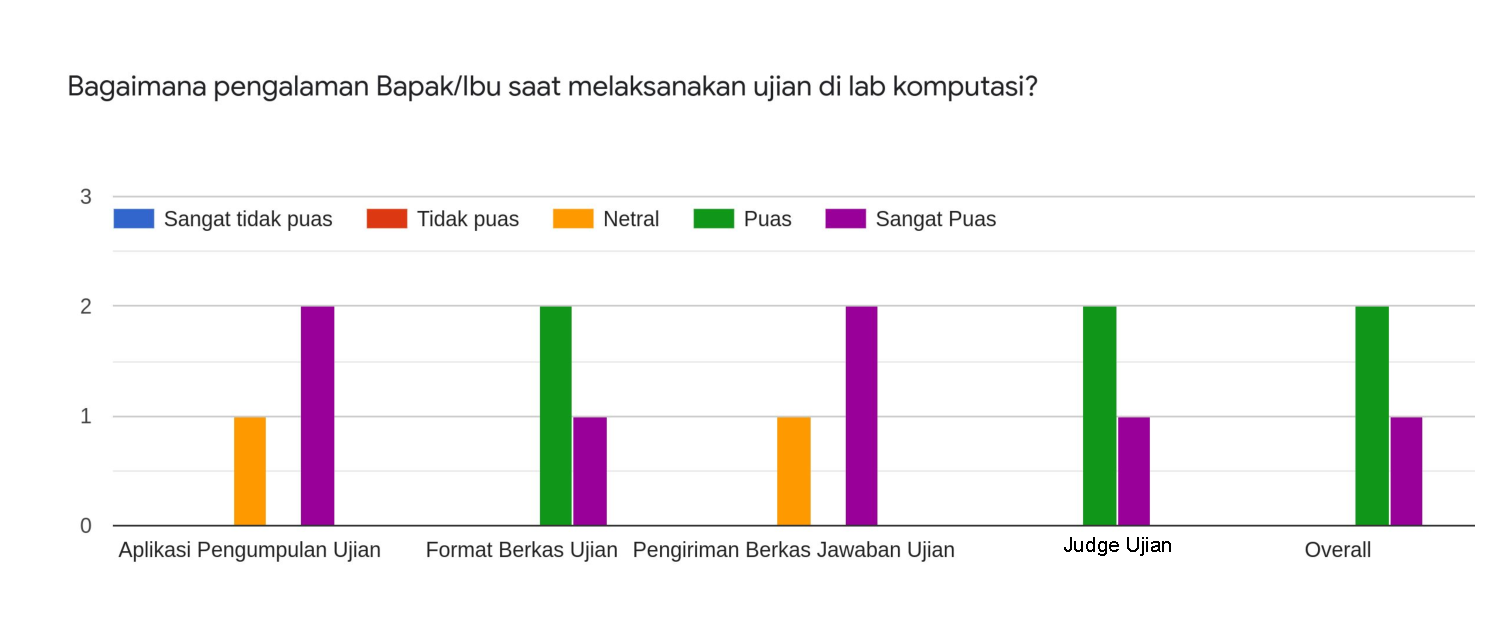
\includegraphics[width=0.6\paperwidth]{Gambar/survey-dosen.pdf}
        \caption{Kuisioner Dosen}
        \label{fig:kuisioner-dosen}
    \end{figure}
    
    Pada kuisioner tersebut, terdapat tiga responden yang memberikan respon.
    Tabel grafik dapat dilihat pada gambar \ref{fig:kuisioner-dosen}.
    Berdasarkan respon-respon yang diberikan, dosen-dosen memiliki
    \textit{feedback} yang positif pada sistem ujian yang saat ini telah
    berjalan. Sehingga sistem ujian yang nantinya akan berjalan pada lab dibuat
    memiliki perubahan seminimal mungkin dari sudut padang dosen.
    
    Pada pertanyaan terakhir, masalah yang dikeluhkan diantaranya:
    \begin{itemize}
        \item Komputer peserta ujian terkadang mengalami \textit{hang}.
        
        \item Hanya ada satu admin yang datang tepat waktu
        
        \item Pertukaran shift kadang membingungkan pengawas, karena pernah
        suatu kali, daftar hadir belum diperbarui
        
        \item Pemberian password kadang masih manual melalui kertas.
        
        \item Kebingungan karena terkadang mahasiswa tidak bisa \textit{submit}
        karena dikatakan "waktu telah habis", tetapi bisa lagi jika
        di-\textit{refresh}.
    \end{itemize}

    
    \subsubsection{Subjek Peserta}
    Formulir kuisioner yang dibagikan untuk peserta ujian memiliki pertanyaan
    sebagai berikut:
    \begin{itemize}
        \item Masalah apa saja yang pernah anda alami?\\
            Tujuan pertanyaan ini adalah untuk mengidentifikasi masalah-masalah
            yang sering dialami oleh peserta ujian. Bentuk jawaban adalah daftar
            kotak yang dapat diceklis.
            \begin{itemize}
                \item "Waktu ujian telah habis"
                \item Waktu ujian tidak terlihat dengan baik/jelas
                \item Daftar tempat duduk yang membingungkan
                \item \textit{Credential}\footnote{informasi \textit{login}}
                untuk \textit{Judge} bermasalah
                \item Tidak memiliki masalah
            \end{itemize}
            
        \item Selain dari masalah tersebut, apakah anda memiliki masalah
        lainnya?\\
            Pertanyaan ini ditujukan untuk mengetahui masalah yang tidak
            diketahui oleh Tim Admin atau tidak terlihat secara langsung pada
            saat survei lapangan. Bentuk jawaban adalah kotak teks panjang.
            
        \item Bagaimana pendapat anda tentang ujian di Lab Komputasi?\\
            Pertanyaan ini ditujukan untuk mengetahui pendapat peserta ujian
            tentang pengalaman ujian di lab. Jawaban berupa skala satu hingga
            lima, dengan satu paling buruk, dan lima paling baik.
            
    \end{itemize}
    Kuisioner ditujukan pada peserta ujian yang pernah mengikuti ujian di lab
    pada saat sistem ini masih digunakan. Kuisioner ini direspon oleh 30
    responden yang terdiri dari beberapa angkatan. Berdasarkan respon yang
    diberikan oleh peserta untuk pertanyaan pertama, secara mayoritas masalah
    yang dialami adalah daftar tempat duduk yang membingungkan, diikuti dengan
    masalah \textit{bug} waktu ujian telah habis (Gambar
    \ref{fig:kuisioner-student-1}).
    \begin{figure}
        \centering
        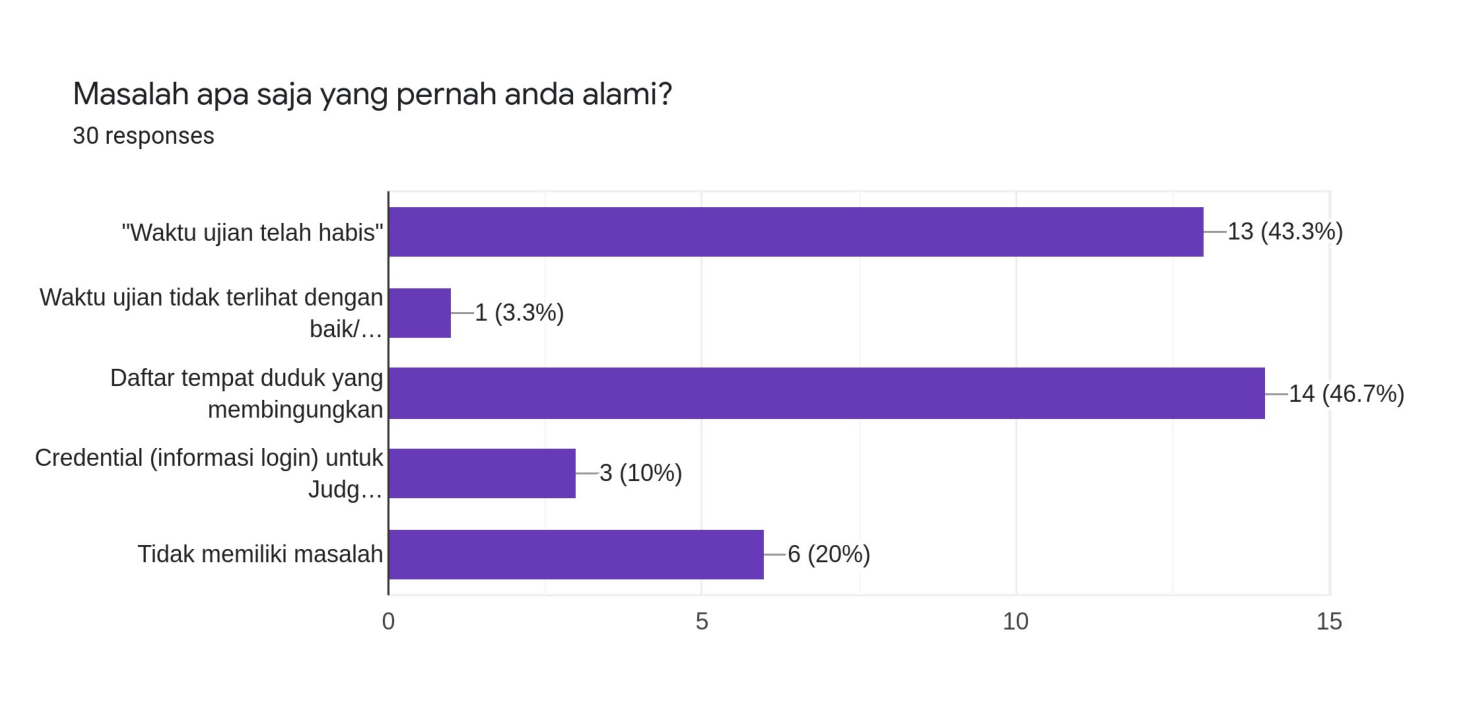
\includegraphics[width=0.7\paperwidth]{Gambar/survey-student.pdf}
        \caption{Respon kuisioner untuk masalah yang telah diketahui pada saat survei}
        \label{fig:kuisioner-student-1}
    \end{figure}
    
    Pada pertanyaan kedua, peserta ujian mengeluhkan beberapa masalah seperti:
    \begin{itemize}
        \item Kadang-kadang sesuatu yang ditulis di papan tulis tidak terlihat
        jelas pada posisi duduk tertentu.
        
        \item Beberapa komputer memiliki masalah jaringan
        
        \item Daftar tempat duduk yang miring dan tanpa garis
        
        \item Waktu ujian yang kurang
        
        \item Komputer \textit{hang}
        
        \item Perangkat lunak yang tidak dapat digunakan ketika ujian
    \end{itemize}
    Dari respon-respon tersebut, tidak semua dapat diselesaikan dengan
    mengimplementasikan solusi pada sistem, sehingga masalah-masalah tersebut
    masuk pada batasan masalah.
    
    Selain itu, secara keseluruhan (lihat Gambar \ref{fig:kuisioner-student-2}),
    peserta ujian memberikan respon yang positif terhadap sistem yang saat ini
    berjalan pada lab. Sehingga pada sisi peserta, perubahan sistem akan dibuat
    seminimal mungkin.
    
    \begin{figure}
        \centering
        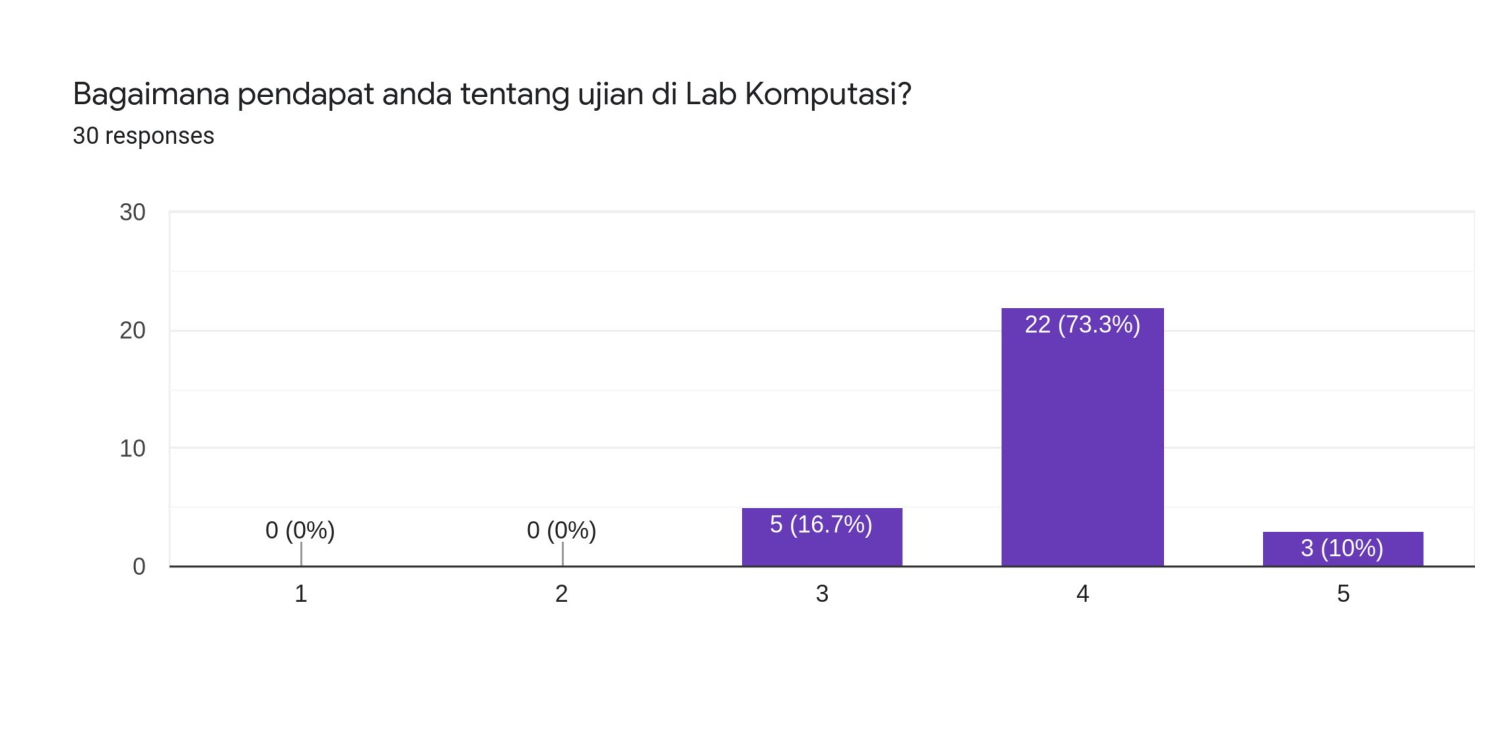
\includegraphics[width=0.7\paperwidth]{Gambar/survey-student-2.pdf}
        \caption{Pendapat peserta ujian pada sistem ujian yang berjalan saat ini}
        \label{fig:kuisioner-student-2}
    \end{figure}
    
\section{Analisis Kebutuhan}
    Berdasarkan survei dan kuisioner yang dilakukan akan dianalisis poin-poin
    masalah. Masalah-masalah tersebut akan dikelompokkan berdasarkan peran yang
    ikut terlibat pada sistem aplikasi ujian.
    
\subsection{Dosen}
    \subsubsection{\textit{Bug} Waktu Telah
        Habis}\label{ref-prob-dosen-bug-waktu} Laporan masalah pertama berasal
        dari sisi Dosen yang mengawasi ujian di lab komputasi. Masalah yang
        sering kali dikeluhkan adalah \textit{bug} waktu telah habis.
        \textit{Bug} ini didapatkan pada saat peserta sudah membuka halaman
        pengumpulan sudah cukup lama tanpa melakukan penyegaran-ulang
        (\textit{refresh}) ataupun pengumpulan (\textit{submission}). Untuk
        mengatasi masalah ini, biasanya Tim Admin akan meminta peserta ujian
        untuk melakukan penyegaran-ulang beberapa kali hingga pesan kesalahan
        tersebut hilang. Setelah diselidiki, bug tersebut disebabkan oleh
        \textit{cache} yang memiliki umur yang pendek. Umur pendek ini
        menyebabkan \textit{cache} kadaluarsa dan dianggap tidak \textit{valid}
        oleh PHP, sehingga memancing aplikasi untuk memunculkan pesan kesalahan
        tersebut, mencegagh peserta untuk mengumpulkan jawaban pada web.
    
    \subsubsection{Pembagian \textit{Password} yang Masih
        Manual}\label{ref-prob-dosen-password} Masalah berikutnya yang Dosen
        berikan pada kuisioner adalah pembagian \textit{password} yang masih
        manual. Pengujian dengan aplikasi khusus adalah salah satu hal yang
        sering dilakukan di Lab Komputasi. Program tersebut biasanya menggunakan
        otentikasi khusus yang tidak dapat diintegrasikan dengan aplikasi Oxam
        utama untuk mencegah kecurangan. Hal ini saat ini diatasi dengan
        membagikan kertas pada tiap meja, atau membagikannya lewat berkas teks
        pada folder ujian. Sistem ini dilakukan dengan cara melakukan penciptaan
        kata sandi acak yang nantinya dimasukkan pada \textit{script} tertentu.
        Selanjutnya Tim Admin akan melakukan pembuatan akun tersebut dengan
        bantuan \textit{script} tersebut, lalu kredensial tersebut nantinya akan
        diolah untuk nantinya dicetak atau pun dipecah menjadi beberapa berkas
        teks sebelum nantinya diedarkan.

    \subsubsection{Daftar Hadir yang Membingungkan
        Pengawas}\label{ref-prob-dosen-daftar-hadir} Berikutnya, daftar hadir
        yang membingungkan pengawas. Pada hal ini, pengawas kebingungan karena
        kesalahan Tim Admin melakukan pendaftaran peserta. Masalah ini nantinya
        akan didalami pada saat pembahasan survei dari Tim Admin.

\subsection{Peserta}
    \subsubsection{Komputer Hang}\label{ref-prob-peserta-kompu-hang} Kuisioner
    kemudian dilakukan juga untuk peserta ujian yang pernah mengikuti ujian di
    lab komputasi. Dari sisi peserta, Masalah yang muncul pada saat ujian adalah
    komputer yang \textit{hang}. Masalah ini muncul secara acak pada saat ujian
    berlangsung. Peserta biasanya akan diminta untuk direlokasi untuk
    mendapatkan komputer yang tidak bermasalah. Peserta akan diberikan waktu
    tambahan sesuai dengan durasi lamanya komputer tidak dapat digunakan hingga
    komputer peserta yang baru diberikan dapat digunakan kembali. Pada kasus
    ini, masalah tersebut masuk dalam batasan masalah yang tidak dapat diatasi.
    
    \subsubsection{Tulisan Pada Papan Tulis yang Tidak
    Terlihat}\label{ref-prob-peserta-papan-tulis} Selain itu, peserta
    mengeluhkan bahwa tulisan yang ada di papan tulis seringkali tidak terlihat.
    Pada ujian, biasanya informasi seperti kata sandi untuk membuka berkas soal,
    informasi \textit{URL} untuk masuk ke dalam sistem informasi, atau revisi
    soal biasanya ditulis pada papan tulis yang ada di depan. Masalah yang
    timbul adalah peserta yang mendapatkan tempat yang terjauh dari papan tulis
    mengaku kesulitan dalam melihat informasi tersebut. Hal ini dinilai tidak
    adil untuk peserta yang duduk dekat dengan papan tulis, sehingga
    dibutuhkannya fitur untuk memberi tahu informasi ini.

\subsection{Tim Admin}
    \subsubsection{Menghapus Berkas yang
    Gagal}\label{ref-prob-admin-berkas-gagal} Dari sisi Tim Admin, survei yang
    dilakukan menghasilkan banyak keluhan dan masukan. Salah satunya, Tim Admin
    mempermasalahkan bahwa mereka tidak dapat menghapus berkas-berkas yang gagal
    di \textit{deploy}. Masalah tersebut biasanya muncul pada saat Tim Admin
    melakukan kesalahan memasukan data pada saat pembuatan ujian pada aplikasi
    Oxam. Tim Admin yang tidak mengetahui kesalahan tersebut dapat saja
    melakukan \textit{deployment} terlebih dahulu sebelum akhirnya menyadari
    bahwa ia telah melakukan kesalahan. Masalah yang dikeluhkan berakar dari
    fodler yang tidak digunakan tersebut membingungkan bagi peserta dan
    berpotensi menjadi celah keamanan untuk mencontek.

    Selain folder, Tim Administrator juga harus menghapus daftar yang ada pada
    database. Setelah diselidiki, masalah timbul dari \textit{record} yang
    ditandai sebagai di hapus dengan mengisi kolom \texttt{isDeleted} menjadi
    \texttt{1}, namun tidak membuat sistem pengumpulan berubah. Masalah yang
    timbul adalah sebagian dari peserta mendapatkan tempat pengumpulan yang
    berbeda dari seharusnya.

    \subsubsection{Pindah Tempat Duduk Peserta}\label{ref-prob-admin-pindah}
    Selain itu, beberapa masalah lainnya adalah pindah tempat duduk peserta.
    Bersinggungan dengan masalah yang dimiliki peserta tentang komputer yang
    \textit{hang} pada \ref{ref-prob-peserta-kompu-hang}, Tim Administator
    memiliki kesulitan untuk melakukan pemindahan komputer karena Aplikasi yang
    saat ini ada memiliki masalah tentang mengubah posisi tempat duduk. Masalah
    yang muncul adalah dibutuhkannya orang untuk melakukan:
    \begin{itemize}
        \item Pemindahan peserta
        \item Pemindahan berkas ujian peserta
        \item Pemindahan \textit{record} pada database Oxam
    \end{itemize}

    Dengan begitu jika terdapat lebih dari seorang peserta yang mengalami
    masalah ini maka dibutuhkan waktu yang sangat lama untuk menyelesaikan
    masalah tersebut.
    
    Selain dari pemindahan tempat duduk tersebut, pemindahan peserta antar
    \textit{shift} juga bermasalah. Peserta ujian yang mengalami bentrok dengan
    ujian yang ada di lab diperbolehkan untuk meminta pemindahan waktu ujian,
    jika ujian tersebut memiliki \textit{shift}. Hal ini dilakukan dengan cara
    mengontak Kepala Lab, lalu Kepala Lab akan mengatur daftar peserta
    sedemikian rupa daftar hadir tersebut sehingga peserta mendapatkan waktu
    yang tepat. Kepala Lab kemudian menginformasikan perubahan tersebut pada Tim
    Admin. Tim Admin yang bertugas kemudian akan membuat daftar hadir, dan
    mengacaknya pada sistem yang saat ini aktif. Masalah yang biasanya timbul
    adalah, pembuatan daftar hadir ini dibuat beberapa hari sebelum ujian,
    sehingga jika terdapat peserta yang meminta untuk berubah jadwal, daftar
    hadir tersebut harus dibuat kembali. Hal ini bersinggungan langsung dengan
    permasalahan yang dosen miliki pada \ref{ref-prob-dosen-daftar-hadir}.

    \subsubsection{Pengiriman Berkas Jawaban
    Otomatis}\label{ref-prob-admin-pengiriman-berkas} Normalnya, setelah ujian
    selesai maka Tim Admin akan mengunduh berkas jawaban tersebut untuk
    dikirimkan ke Dosen Koordinator. Tim Admin akan mengakses aplikasi Oxam,
    lalu mengunduh berkas jawaban ujian dan mengirimnya secara manual ke Dosen
    Koordinator mata kuliah tersebut. Masalah yang muncul adalah tidak setiap
    kali ujian Tim Admin ingat untuk mengirimkan berkas.
    
    \subsubsection{NPM Jenis Baru}\label{ref-prob-admin-npm-baru} Peserta yang
    menjalani ujian praktik pada lab komputasi adalah mahasiswa. Bergantinya
    sistem informasi akademik kampus berdampak pada pergantian format NPM yang
    dimiliki oleh mahasiswa. NPM pada mahasiswa memiliki format tertentu yang
    dapat menginformasikan asal dari mahasiswa tersebut. Format yang dimiliki
    oleh 
    
    \subsubsection{Kode Matakuliah Baru}\label{ref-prob-admin-kode-mk-baru}
    Kurikulum yang saat ini ada memikili kode matakuliah yang baru. Masalah yang
    muncul adalah sistem aplikasi yang lama tidak memiliki admin panel untuk
    melakukan manajemen mata kuliah yang baru.
    
    \subsubsection{Timer yang tidak
    terintegrasi}\label{ref-prob-admin-timer-integrated} Pada saat pelaksanaan
    ujian, Tim Admin menggunakan timer yang disediakan oleh sistem operasi
    Windows. Masalah yang timbul adalah buka dan tutupnya tempat pengumpulan
    ujian tidak berjalan bersamaan dengan timer. Sebagai contoh, pada saat timer
    menunjukan waktu sudah habis, peserta masih dapat mengumpulkan berkas ujian.
    
    
\section{Analisis Fitur Aplikasi}
    Berdasarkan survei yang dilakukan dan kuisioner yang disebar, didapatkan
    beberapa masalah yang menandakan bahwa aplikasi pendukung ujian di lab
    komputasi belum efektif membantu pelaksanaan ujian. Masalah-masalah tersebut
    akan diselesaikan dengan merekayasa ulang aplikasi yang telah ada pada
    sistem yang lama. Rekayasa ulang tersebut dilakukan dengan bantuan
    \textit{framework} agar sumber kode yang dibuat dapat dirawat oleh tim
    Admin.
    
    Fitur-fitur yang akan di rekayasa ulang akan didetilkan pada tabel
    \ref{tab:table-daftar-fitur}.
    
    \begin{table}[H]
        \centering
        \begin{tabular}{|p{4.5cm}|l|l|l|}
        \hline
        Nama Fitur & Referensi Masalah & Asal Fitur & Status\\
        \hline
        Membuat, melihat, mengubah, menghapus ujian & - & Lama & Rekayasa Ulang
        \\
        \hline
        Melihat, mencetak daftar peserta yang sudah diacak & - & Lama & Rekayasa
        Ulang \\
        \hline
        Mengunggah dan mengunduh jawaban & - & Lama & Rekayasa Ulang \\
        \hline
        Timer (tidak terintegrasi)  & \ref{ref-prob-admin-timer-integrated} &
        Lama & Rekayasa Ulang \\
        \hline
        Notifikasi & \ref{ref-prob-dosen-password},
        \ref{ref-prob-peserta-papan-tulis} & Baru & Diimplementasi \\
        \hline
        Pemindahan tempat duduk peserta & \ref{ref-prob-peserta-kompu-hang},
        \ref{ref-prob-admin-pindah} & Baru & Diimplementasi \\
        \hline
        Pengiriman berkas otomatis & \ref{ref-prob-admin-pengiriman-berkas} &
        Baru & Diimplementasi \\
        \hline
        NPM \textit{Converter} & \ref{ref-prob-admin-npm-baru} & Baru &
        Diimplementasi \\
        \hline
        Admin Panel & \~{} & Baru & Diimplementasi \\
        \hline
        \textit{Bug fix} & \ref{ref-prob-dosen-bug-waktu},
        \ref{ref-prob-admin-berkas-gagal}  & - & Diimplementasi \\
        \hline
        \end{tabular}
        \caption{Daftar fitur yang akan diimplementasi dan direkayasa ulang}
        \label{tab:table-daftar-fitur}
    \end{table}
    
    \subsection{Timer Tidak Terintegrasi}
        Sesuai dengan kebutuhan yang dijelaskan pada
        \ref{ref-prob-admin-timer-integrated}, timer akan diimplementasi secara
        terintegrasi. Timer nantinya akan menutup tempat jawaban pada saat waktu
        telah habis. Timer harus dapat mengatur buka tutupnya tempat pengumpulan
        jawaban peserta.
    
    \subsection{Notifikasi}
        Fitur pertama yang ingin ditambahkan adalah sistem notifikasi. Fitur ini
        nantinya akan menyelesaikan masalah pada keluhan kata sandi yang
        disebarkan manual (\ref{ref-prob-dosen-password}), dan informasi yang
        dituliskan di papantulis tidak terlihat
        (\ref{ref-prob-peserta-papan-tulis}). Dosen pengawas nantinya dapat
        membuat buah notifikasi baru untuk peserta dan peserta dapat langsung
        melihat notifikasi tersebut pada tempat pengumpulan.

    \subsection{Pemindahan Tempat Duduk Peserta}
        Fitur kedua yang ingin ditambahkan adalah fitur pemindahan tempat duduk
        peserta, atau peserta antar \textit{shift}. Fitur ini nantinya akan
        menyelesaikan masalah peserta yang mengalami \textit{hang} pada saat
        ujian berlangsung (\ref{ref-prob-peserta-kompu-hang}) dan Tim Admin yang
        ingin memindahkan tempat duduk peserta, atau peserta antar
        \textit{shift} (\ref{ref-prob-admin-pindah}). Fitur ini nantinya hanya
        akan dapat digunakan oleh Tim Admin. Dosen pengawas diharapkan untuk
        mengkontak Tim Admin untuk melakukan perpindahan untuk memastikan
        komputer yang baru akan memiliki kemungkinan bermasalah yang lebih
        kecil.

    \subsection{Pengiriman berkas otomatis}
        Fitur lainnya adalah perngiriman berkas otomatis. Fitur ini untuk
        menyelesaikan masalah pada pengiriman berkas jawaban ujian oleh Tim
        Admin (\ref{ref-prob-admin-pengiriman-berkas}). Pada dasarnya fitur ini
        dapat implementasi dengan cara membuat \textit{cronjob} setiap menit
        yang nantinya mengecek apakah terdapat berkas ujian yang dapat di kirim.
        Pengiriman dapat berlangsung secara otomatis lewat email.

    \subsection{NPM \textit{Converter}} NPM \textit{Converter} nantinya akan
        mengabstraksi seluruh NPM yang saat ini aktif di sistem UNPAR. Abstraksi
        tersebut nantinya diharapkan dapat menstandarisasi dua format yang saat
        ini berjalan.
        
    \subsection{Admin Panel}
        Admin panel ditambahkan dengan tujuan agar dapat memanajemen seluruh
        entitas database pendukung ujian. Sebagai contoh, penambahan atau
        penghapusan mata kuliah. Saat ini, pada sistem yang aktif tidak terdapat
        tempat untuk menambahkan atau menghapus mata kuliah.
    
    \subsection{Bug \textit{fix}} Implementasi sisanya, terdapat beberapa
        masukan yang dapat dilakukan, yaitu untuk menyelesaikan masalah tentang
        \textit{bug} waktu ujian telah habis (\ref{ref-prob-dosen-bug-waktu})
        dapat diimplementasi dengan melakukan authentikasi berdasarkan IP yang
        tidak disimpan menggunakan \textit{cache} atau \textit{session}. Hal ini
        memperkecil masalah \textit{cache} atau \textit{session} yang kadaluarsa
        karena waktu yang diberikan terlalu kecil. Sehingga setiap kali koneksi
        dijalankan dari klien ke \textit{server}, server akan langsung mengecek
        IP tersebut dengan yang ada di database melakukan apapun.

\section{Analisis Pemilihan Framework dan Library}
%- Pake framework biar daapt di extend oleh penerus
Penggunaan \textit{framework} diharapkan dapat membuat aplikasi dikembangkan
lebih lanjut oleh penerus Tim Admin berikutnya. Sifat \textit{framework} yang
dapat digunakan-ulang dan modular membuat \textit{framework} memiliki pola yang
dapat dipelajari dengan cepat. Memungkinkan Tim Admin untuk dapat menambahkan
fitur baru dengan lebih cepat. 

Berdasarkan survei yang dilakukan oleh StackOverflow pada tahun
2018\cite{stackoverflow:survey-2018} dan 2019\cite{stackoverflow:survey-2019},
PHP adalah salah satu bahasa yang mayoritas digunakan oleh pengembang aplikasi
web. Dengan banyaknya pengguna bahasa tersebut, maka komunitas, \textit{library}
dan firum akan lebih besar. Pilihan tersebut dinilai lebih menguntungkan karena
pengembang hanya perlu mempelajari cara menggunakan \textit{library} tersebut
tanpa harus mengimplementasi algoritmanya dari dasar. Dengan begitu banyaknya
pilihan yang ada, developer yang ingin menambahkan fitur tersebut dapat lebih
berfokus untuk mengimplementasi fitur tersebut.

\subsection{FatFree Framework}

\begin{figure}[H]
    \centering
    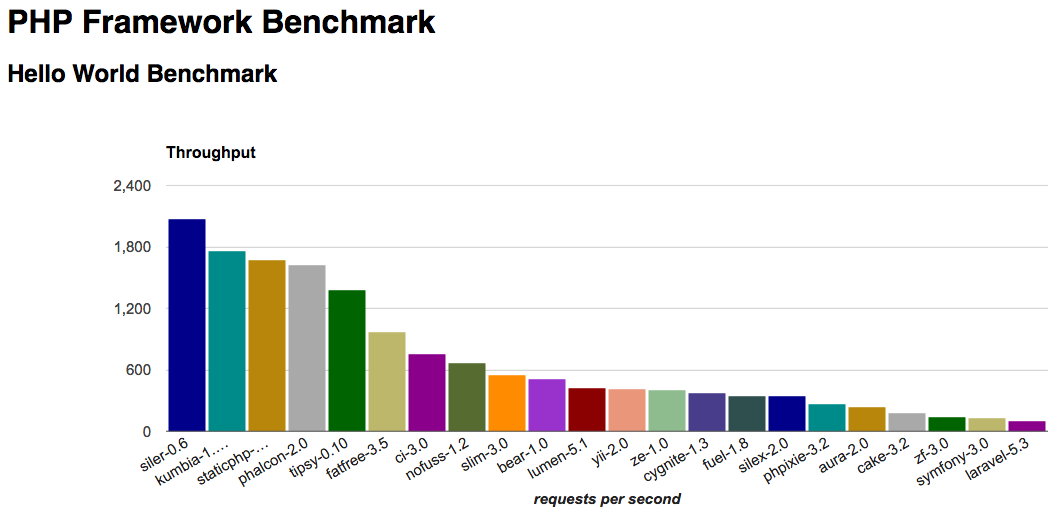
\includegraphics[width=0.6\paperwidth]{Gambar/php-framework-benchmark-20170214.png}
    \caption{Hasil \textit{benchmark} terhadap beberapa \textit{framework} pada
        bahasa pemrograman PHP\protect\cite{kenjis:framework-benchmark}. (Lebih
        tinggi lebih baik)}
    \label{fig:chart-benchmark-php-framework}
\end{figure}

%- Karena penggunaan fleksibel
Beberapa \textit{framework} memiliki sifat yang fleksibel, sehingga memungkinkan
developer mengadopsi framework tersebut dengan gaya mereka masing-masing.
Fat-Free framework tidak memiliki pola pemrograman yang pasti, namun sistem
mereka dirancang agar dapat digunakan pada tipe pola pemrograman apapun. Kontras
dengan framework besar seperti Laravel, atau Code Igniter. Fat-free sendiri
dengan jelas menuliskan untuk menggunakan gaya apapun yang pengembang
butuhkan\footnote{https://fatfreeframework.com/3.6/getting-started\#EnoughSaid-SeeForYourself}.
 
Dengan sifat analisis kebutuhan yang cepat, maka penggunaan framework yang kecil
dan ringan dibutuhkan. Selain itu dengan kebutuhan yang mengharuskan
implementasi cukup fleksibel untuk kemudian hari dikembangkan lebih lanjut, maka
FatFree Framework atau F3 akan digunakan untuk penelitan ini.

\subsection{React.js}
    Menurut survey yang dilakukan oleh StackOverflow pada tahun 2019, Reactjs
    adalah salah satu \textit{framework} javascript yang paling banyak digunakan
    pada
    web\footnote{https://insights.stackoverflow.com/survey/2019{\#}technology-{\_}-web-frameworks}.
    Selain itu menurut survey tersebut, Reactjs adalah salah satu framework yang
    paling disukai oleh pengembang. Dengan dua alasan tersebut penelitian ini
    menggunakan Reactjs sebagai \textit{framework} Frontend.

\subsection{CI/CD}
    Penggunaan \textit{library} React pada front-end membutuhkan tahap tambahan
    untuk melakukan \textit{build} sebelum subsistem dapat dijalankan di
    peramban pengguna. Adanya tahap tambahan ini membuat penelitian ini
    membutuhkan sebuah sistem \textit{build} terpusat untuk mempermudah
    mengelola kode sumber yang akan di-\textit{deploy} pada peladen produksi.
    Sistem build ini akan diimplementasi dengan menggunakan teknologi CI/CD yang
    disediakan oleh penyedia penyimpanan kode sumber, GitLab.
    
    Sistem CI/CD nantinya harus dapat berjalan hampir otomatis seluruhnya untuk
    menyederhanakan alur pengembangan aplikasi. Sistem CI/CD ini diharapkan
    untuk mempermudah pekerjaan pengembang untuk melakukan \textit{build} dengan
    standar produksi dengan package dan modules untuk development tidak
    diikutkan pada hasil \textit{build}. Harapan lainnya adalah dengan adanya
    CI/CD ini, pengembang dapat menambahkan \textit{routine} apapun yang
    dibutuhkan dikemudian hari.

\section{Analisis Pengguna}

\begin{figure}
    \centering
    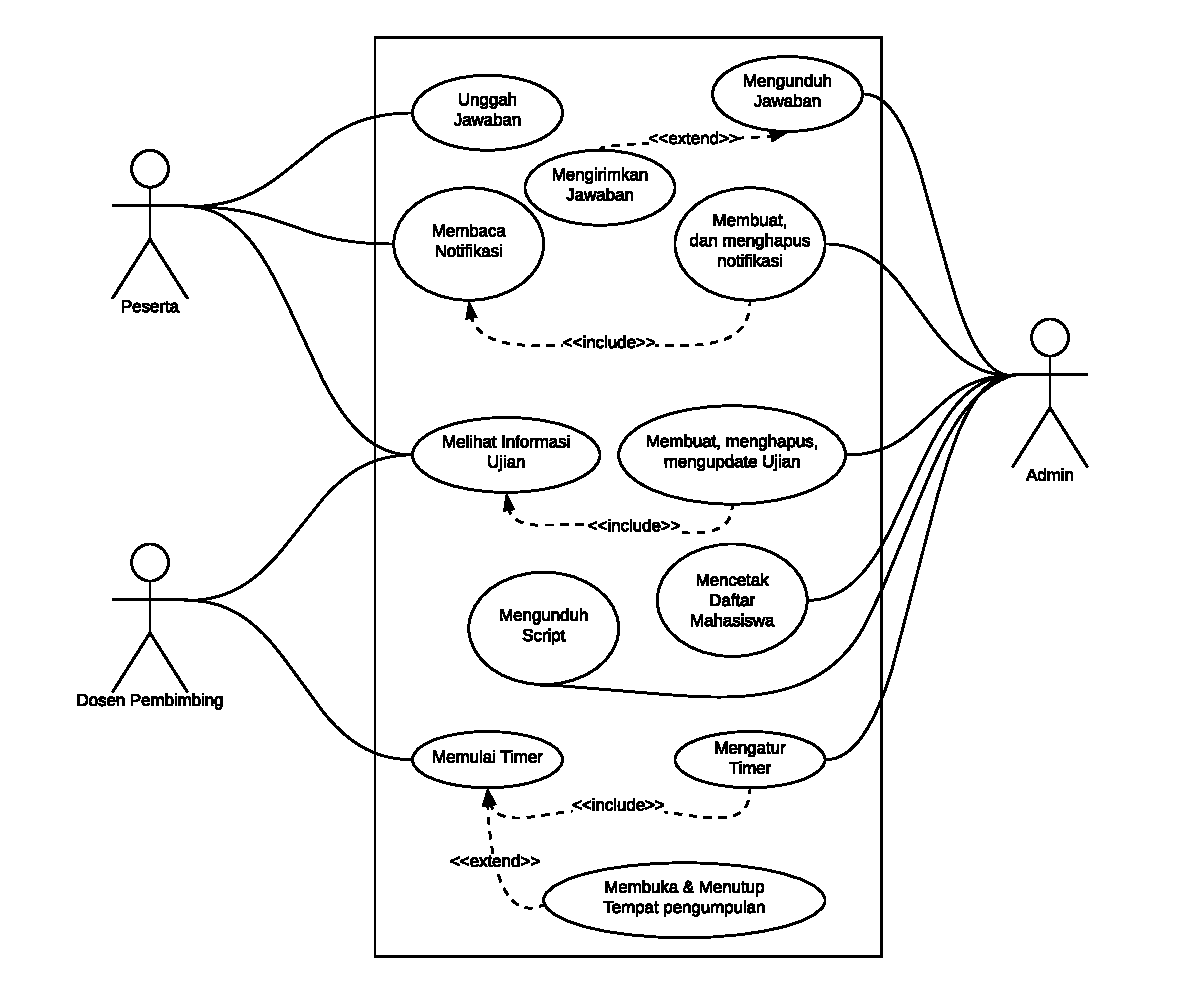
\includegraphics[width=0.75\paperwidth]{Gambar/diagram-usecase.pdf}
    \caption{Diagram \textit{Use Case}}
    \label{fig:my_label}
\end{figure}

Pengguna sistem ini nantinya akan terdiri dari dua pihak. Pihak pertama, Pihak
Administrator. Administrator adalah salah satu pengguna yang memiliki hak akses
penuh terhadap sistem manajemen ujian. Pihak ini nantinya akan digunakan oleh
tim Administrator Laboratorium. Tim ini nantinya akan membantu menyiapkan ujian,
ruangan ujian, dan berkas-berkas administrasi yang nantinya digunakan selama
ujian.

Pihak berikutnya, yaitu pihak kedua, nantinya digunakan oleh peserta ujian.
Nantinya peserta ini akan menggunakan aplikasi ini untuk mengumpulkan berkas
jawaban ujian. Peserta ujian hanya akan dapat mengakses halaman pengumpulan.
Pada halaman ini nantinya peserta ujian hanya dapat melihat informasi ujian,
informasi ruangan, format nama berkas ujian, dan waktu sisa ujian. Waktu ini
disingkronisasi dengan waktu yang terdapat pada server dan layar proyektor.